% Book pp. 102-111 (PDF pp. 103-112)
\section{Sketching Polynomial Functions with Degrees Higher Than 2}

\begin{enumerate}
  \item In mathematics, the terms ``sketch'' and ``draw'' have distinct meanings.
  \item Sketch is a rough representation of a graph or function without precise
  measurements, used to illustrate its behaviour. It often lacks scales and
  coordinates.
  \item Draw, on the other hand, creates a more accurate representation with
  specific values, scales, and tools, providing a detailed visualization of a
  mathematical function or data set.
\end{enumerate}

We will be sketching polynomial functions with a degree higher than 2.

These will be cubics, quartics etc.

To sketch a polynomial of degree greater than 2, for example, $ax^3 + bx^2 + cx + d$,
we:

\textbf{Step 1:} Determine the sign ($+$ or -) of \textbf{a}; if a $>$ 0 or a $<$ 0

If a $<$ 0, the curve will have the shape:
\booknote[S3-05]{the book prints ``a $<$ 0'' above both Figure 3.1 and
Figure 3.2, and both figures show the shape for $a > 0$ (rising from bottom left
to top right). The first should read ``a $>$ 0''; the second figure should be the
reflected shape, falling from top left to bottom right.}
\begin{center}
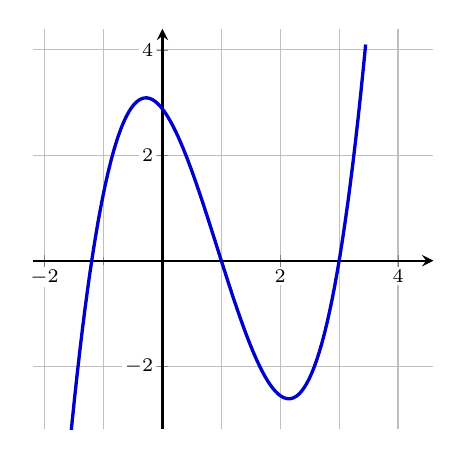
\begin{tikzpicture}
\begin{axis}[
  width=0.55\linewidth, height=0.55\linewidth,
  axis lines=middle, grid=both, minor tick num=1,
  xmin=-2.2, xmax=4.6, ymin=-3.2, ymax=4.4,
  xtick={-2,0,2,4}, ytick={-2,2,4},
  tick label style={font=\scriptsize}, ticklabel style={fill=white, inner sep=1pt},
  axis line style={thick},
]
\addplot[blue!80!black, very thick, samples=120, domain=-1.75:3.45]
  {0.8*(x+1.2)*(x-1)*(x-3)};
\end{axis}
\end{tikzpicture}
\end{center}
\figcaption{3.1}{Curve of a polynomial}

If a $<$ 0, the curve will have the shape:
\begin{center}
\begin{tikzpicture}[scale=0.8]
  \draw[-{Stealth}] (-4.2,0) -- (4.2,0) node[above left, font=\scriptsize] {$x$};
  \draw[-{Stealth}] (0,-2.6) -- (0,2.6) node[below right, font=\scriptsize] {$y$};
  \node[font=\scriptsize, above right] at (-4.1,0) {$x'$};
  \node[font=\scriptsize, right] at (0,-2.4) {$y'$};
  \draw[red!70, thick, samples=100, domain=-3.9:3.8, smooth]
    plot (\x, {0.11*\x*\x*\x - 0.95*\x});
\end{tikzpicture}
\end{center}
\figcaption{3.2}{Curve of a polynomial}

\textbf{Step 2:} Use the factor theorem or any known method to find the zeros of the
polynomial

\textbf{Step 3:} Find the y- intercept of the function by substituting x $=$ 0 into the
given polynomial function. (Note that this equates to the constant.)

\textbf{Step 4:} Find the intervals of the curve based on the zeros obtained

\textbf{Step 5:} Sketch the curve.

Individually, or in groups, let's use the steps for sketching polynomials to solve
the examples below.

\begin{example}{Example 3.6}
Sketch the curve $2x^3 + 3x^2 - 5x - 6$

\solution
\textbf{Step 1:} a is 2, which is greater than 0. Therefore, we know the shape that the
curve will take. The extremes will go from bottom left to top right.

\textbf{Step 2:} Using the factor theorem, the factors of the constant, - 6 are
$\pm 1, \pm 2, \pm 3, \pm 6$

Testing when x $=$ - 1, we have:

$2(-1)^3 + 3(-1)^2 - 5(-1) - 6 = -2 + 3 + 5 - 6 = 0$

Which means $(x + 1)$ is a factor.

We can use long division to find the other factors.
\[
\begin{array}{r@{\;}r}
 & 2x^2 + x - 6 \\ \cline{2-2}
x + 1\,\big) & 2x^3 + 3x^2 - 5x - 6 \\
 & \underline{-(2x^3 + 2x^2 + 0 + 0)} \\
 & x^2 - 5x - 6 \\
 & \underline{-(x^2 + x + 0)} \\
 & (-6x - 6) \\
 & \underline{-6x - 6}
\end{array}
\]
Factorising:

$2x^2 + x - 6$

$2x^2 + 4x - 3x - 6$

$2x(x + 2) - 3(x + 2)$

$(2x - 3)(x + 2)$

Factors are:

$(x + 1)(2x - 3)(x + 2)$

The zeros:

$(x + 1)(2x - 3)(x + 2) = 0$

$x = -1$, $x = -2$, $x = \frac{3}{2}$

\textbf{Step 3:} y intercept

When x $=$ 0

$2(0)^3 + 3(0)^2 - 5(0) - 6 = -6$

\textbf{Step 4}: finding the intervals using the zeros
\begin{center}
\begin{tikzpicture}[x=2.2cm]
  \draw[{Stealth}-{Stealth}, thick] (-0.7,0) -- (3.7,0);
  \foreach \x/\l in {0.5/{(-2, 0)}, 1.5/{(-1, 0)}, 2.5/{(1.5, 0)}} {
    \draw[thick] (\x,0.15) -- (\x,-0.15);
    \node[below, font=\scriptsize\bfseries] at (\x,-0.2) {\l};
  }
\end{tikzpicture}
\end{center}
The intervals are:
\begin{enumerate}
  \item $-2 < x$
  \item $-2 < x < -1$
  \item $-1 < x < 1.5$
  \item $x > 1.5$
\end{enumerate}
\booknote[S3-06]{the first interval is printed as $-2 < x$ (and $-1 < x$ in
Examples 3.7 and 3.8); the interval to the left of the first zero is $x < -2$
(respectively $x < -1$), as the table headings below show.}

Next is to determine the signs or test for the signs in each of the intervals obtained

\begin{center}
\small\renewcommand{\arraystretch}{1.2}
\begin{tabular}{|p{0.2\linewidth}|p{0.15\linewidth}|p{0.15\linewidth}|p{0.15\linewidth}|p{0.15\linewidth}|}
\hline
\textbf{Interval} & {\boldmath$-2 > x$} & {\boldmath$-2 < x < -1$} & {\boldmath$-1 < x < 1.5$} & {\boldmath$x > 1.5$} \\
\hline
Chosen values (you can choose any number within the interval)
& \centering\textbf{-3} & \centering\textbf{-1.5} & \centering\textbf{1} & \centering\textbf{2} \tabularnewline
\hline
$y$ value (substitute your chosen number into the given function)
& \centering $2(-3)^3 + 3(-3)^2 - 5(-3) - 6$ \par\medskip \textbf{= -18}
& \centering $2(-1.5)^3 + 3(-1.5)^2 - 5(-1.5) - 6$ \par\medskip \textbf{= 1.5}
& \centering $2(1)^3 + 3(1)^2 - 5(1) - 6$ \par\medskip \textbf{= -6}
& \centering $2(2)^3 + 3(2)^2 - 5(2) - 6$ \par\medskip \textbf{= 12} \tabularnewline
\hline
Sign & \centering Negative & \centering Positive & \centering Negative & \centering Positive \tabularnewline
\hline
Behaviour of curve & Below $x$ - axis & Above $x$ - axis & Below $x$ - axis & Above $x$ - axis \\
\hline
\end{tabular}
\end{center}

\textbf{Step 5:} sketch the curve
\begin{center}
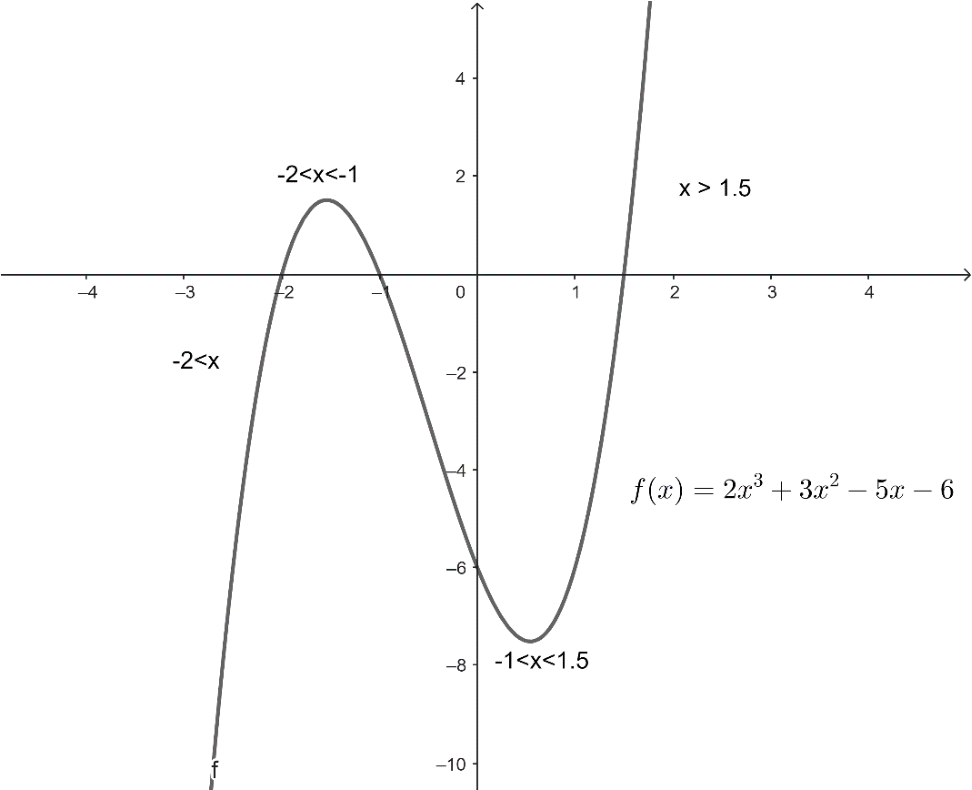
\includegraphics[width=0.75\linewidth]{figures/fig3-3.png}
\end{center}
\figcaption{3.3}{Curve of $2x^3 + 3x^2 - 5x - 6$}
\end{example}

\begin{example}{Example 3.7}
Sketch the curve $x^3 - 6x^2 + 5x + 12$

\solution
\textbf{Step 1:} a is 1 which is greater than 0. This means we know the shape the curve
will take.

\textbf{Step 2:} Using the factor theorem, the factors of the constant, 12 are
$\pm 1, \pm 2, \pm 3, \pm 4 \pm 6, \pm 12$

Testing when x $=$ - 1, we have:

$(-1)^3 - 6(-1)^2 + 5(-1) + 12$

$-1 - 6 - 5 + 12 = 0$

Which means $(x + 1)$ is a factor

We can use long division to find the other factors.
\[
\begin{array}{r@{\;}r}
 & x^2 - 7x + 12 \\ \cline{2-2}
x + 1\,\big) & x^3 - 6x^2 + 5x + 12 \\
 & \underline{-(x^3 + x^2 + 0 + 0)} \\
 & -7x^2 + 5x + 12 \\
 & (-7x^2 - 7x + 12) \\
 & 12x + 12 \\
 & \underline{-(12x + 12)} \\
 & 0
\end{array}
\]
\booknote[S3-07]{the line being subtracted is printed as $(-7x^2 - 7x + 12)$,
without the minus sign; it should be $-(-7x^2 - 7x + 0)$. The remainder line
$12x + 12$ and the quotient are correct.}

Factorising:

$x^2 - 7x + 12$

$x^2 - 4x - 3x + 12$

$x(x - 4) - 3(x - 4)$

$(x - 3)(x - 4)$

Factors are

$(x + 1)(x - 3)(x - 4)$

The zeros

$(x + 1)(x - 3)(x - 4) = 0$

$x = -1$, $x = 3$, $x = 4$

\textbf{Step 3:} $y$ intercept

At x $=$ 0

$(0)^3 - 6(0)^2 + 5(0) + 12 = 12$

\textbf{Step 4}: finding the intervals using the zeros
\begin{center}
\begin{tikzpicture}[x=2.2cm]
  \draw[{Stealth}-{Stealth}, thick] (-0.7,0) -- (3.7,0);
  \foreach \x/\l in {0.5/{(-1, 0)}, 1.5/{(3, 0)}, 2.5/{(4, 0)}} {
    \draw[thick] (\x,0.15) -- (\x,-0.15);
    \node[below, font=\scriptsize\bfseries] at (\x,-0.2) {\l};
  }
\end{tikzpicture}
\end{center}
The interval are
\begin{enumerate}
  \item $-1 < x$
  \item $-1 < x < 3$
  \item $3 < x < 4$
  \item $x > 4$
\end{enumerate}
\booknote[S3-06]{see the note at Example 3.6: the first interval should be $x < -1$.}

Next is to determine the signs or test for the signs in each of the intervals obtained

\noindent\textbf{Table 3.1:} Test for signs in each of the intervals obtained
\begin{center}
\small\renewcommand{\arraystretch}{1.2}
\begin{tabular}{|p{0.2\linewidth}|p{0.15\linewidth}|p{0.15\linewidth}|p{0.15\linewidth}|p{0.15\linewidth}|}
\hline
\textbf{Interval} & {\boldmath$-2 > x$} & {\boldmath$-2 < x < -1$} & {\boldmath$-1 < x < 1.5$} & {\boldmath$x > 1.5$} \\
\hline
Chosen values (you can choose any number within the interval)
& \centering\textbf{-2} & \centering\textbf{1} & \centering\textbf{3.5} & \centering\textbf{5} \tabularnewline
\hline
y value (substitute your chosen number into the given function)
& \centering $(-2)^3 - 6(-2)^2 + 5(-2) + 12$ \par\medskip \textbf{= -30}
& \centering $(1)^3 - 6(1)^2 + 5(1) + 12$ \par\medskip \textbf{= 12}
& \centering $(3.5)^3 - 6(3.5)^2 + 5(3.5) + 12$ \par\medskip \textbf{= -1.125}
& \centering $2(5)^3 + 3(5)^2 - 5(5) - 6$ \par\medskip \textbf{= 294} \tabularnewline
\hline
Sign & \centering Negative & \centering Positive & \centering Negative & \centering Positive \tabularnewline
\hline
Behaviour of curve & Below x - axis & Above x - axis & Below x - axis & Above x - axis \\
\hline
\end{tabular}
\end{center}
\booknote[S3-08]{Table 3.1 repeats the interval headings of Example 3.6
($-2 > x$, $-2 < x < -1$, $-1 < x < 1.5$, $x > 1.5$) instead of $x < -1$,
$-1 < x < 3$, $3 < x < 4$, $x > 4$, and the last column evaluates the Example 3.6
polynomial $2x^3 + 3x^2 - 5x - 6$ at $x = 5$ (giving 294) instead of
$x^3 - 6x^2 + 5x + 12$, which gives 12. The sign, Positive, is unchanged.}

\begin{center}
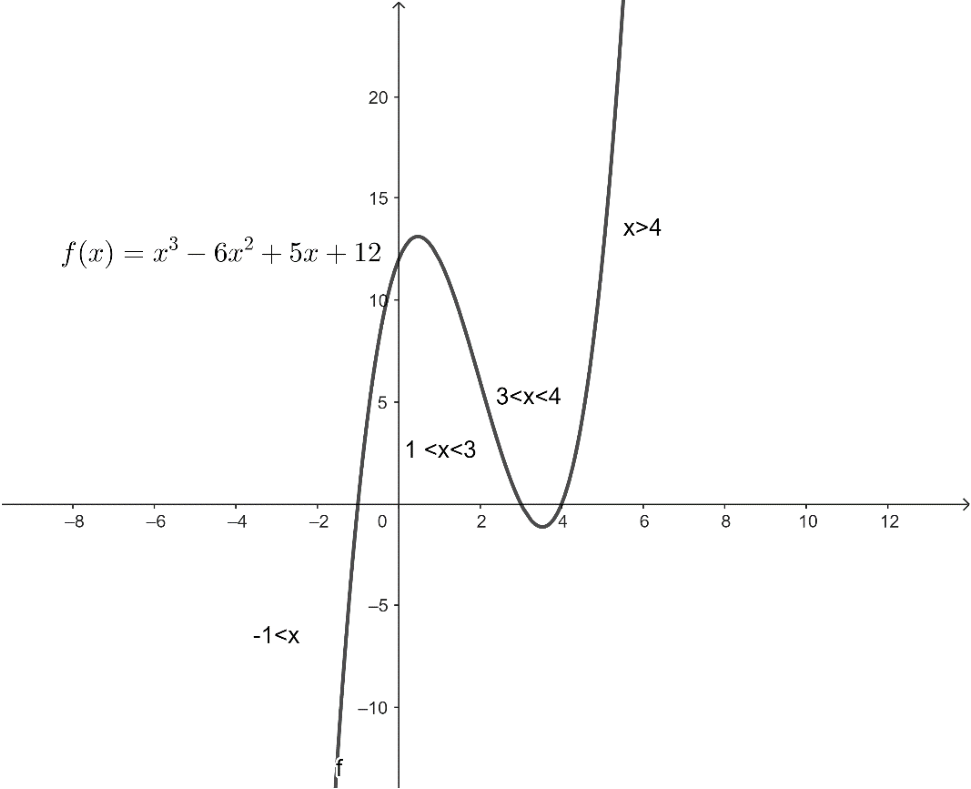
\includegraphics[width=0.75\linewidth]{figures/fig3-4.png}
\end{center}
\figcaption{3.4}{Curve of $x^3 - 6x^2 + 5x + 12$}
\end{example}

\begin{example}{Example 3.8}
Sketch the curve $-x^3 + 4x^2 - x - 6$

\solution
\textbf{Step 1:} a is -1 which is less than 0. This means that the extremes of the graph
go from top left to bottom right.

\textbf{Step 2:} Using the factor theorem, the factors of the constant, -6 are
$\pm 1, \pm 2, \pm 3, \pm 6$

Testing when x $=$ 2, we have:

$-(2)^3 + 4(2)^2 - 2 - 6 = -8 + 16 - 2 - 6 = 0$

Which means $(x - 2)$ is a factor.

We can use long division to find the other factors.
\[
\begin{array}{r@{\;}r}
 & -x^2 + 2x + 3 \\ \cline{2-2}
x - 2\,\big) & -x^3 + 4x^2 - x - 6 \\
 & \underline{-(-x^3 + 2x^2 + 0 + 0)} \\
 & 2x^2 - x - 6 \\
 & -(2x^2 - 4x - 6) \\
 & 3x - 6 \\
 & \underline{-(3x - 6)} \\
 & 0
\end{array}
\]
\booknote[S3-09]{the second subtraction is printed as $-(2x^2 - 4x - 6)$; the
line being subtracted is $2x(x - 2) = 2x^2 - 4x + 0$. The remainder $3x - 6$
and the quotient are correct.}

Factorising:

$-x^2 + 2x + 3$

$-x^2 + 3x - x + 3$

$-x(x - 3) - 1(x - 3)$

$(-x - 1)(x - 3)$

Factors are

$(x - 2)(x - 3)(-x - 1)$

The zeros

$(x - 2)(x - 3)(-x - 1) = 0$

$x = -1$, $x = 3$, $x = 2$

\textbf{Step 3:} y intercept:

When x $=$ 0

$-(0)^3 + 4(0)^2 - (0) - 6 = -6$

\textbf{Step 4}: finding the intervals using the zeros
\begin{center}
\begin{tikzpicture}[x=2.2cm]
  \draw[{Stealth}-{Stealth}, thick] (-0.7,0) -- (3.7,0);
  \foreach \x/\l in {0.5/{(-1, 0)}, 1.5/{(2, 0)}, 2.5/{(3, 0)}} {
    \draw[thick] (\x,0.15) -- (\x,-0.15);
    \node[below, font=\scriptsize\bfseries] at (\x,-0.2) {\l};
  }
\end{tikzpicture}
\end{center}
The intervals are
\begin{enumerate}
  \item $-1 < x$
  \item $-1 < x < 2$
  \item $2 < x < 3$
  \item $x > 3$
\end{enumerate}
\booknote[S3-06]{see the note at Example 3.6: the first interval should be $x < -1$.}

Next is to determine the signs or test for the signs in each of the intervals obtained

\noindent\textbf{Table 3.2:} Test for signs in each of the intervals obtained
\begin{center}
\small\renewcommand{\arraystretch}{1.2}
\begin{tabular}{|p{0.2\linewidth}|p{0.15\linewidth}|p{0.15\linewidth}|p{0.15\linewidth}|p{0.15\linewidth}|}
\hline
\textbf{Interval} & {\boldmath$-1 > x$} & {\boldmath$-1 < x < 2$} & {\boldmath$2 < x < 3$} & {\boldmath$x > 3$} \\
\hline
Chosen values (you can choose any number within the interval)
& \centering\textbf{-3} & \centering\textbf{1} & \centering\textbf{2.5} & \centering\textbf{4} \tabularnewline
\hline
y value (substitute your chosen number into the given function)
& \centering $-(-3)^3 + 4(-3)^2 - (-3) - 6$ \par\medskip \textbf{= 60}
& \centering $-(1)^3 + 4(1)^2 - (1) - 6$ \par\medskip \textbf{= -4}
& \centering $-(2.5)^3 + 4(2.5)^2 - (2.5) - 6$ \par\medskip \textbf{= 0.875}
& \centering $-(4)^3 + 4(4)^2 - (4) - 6$ \par\medskip \textbf{= -10} \tabularnewline
\hline
Sign & \centering Positive & \centering Negative & \centering Positive & \centering Negative \tabularnewline
\hline
Behaviour of curve & Above $x$ - axis & Below $x$ - axis & Above $x$ - axis & Below $x$ - axis \\
\hline
\end{tabular}
\end{center}

\begin{center}
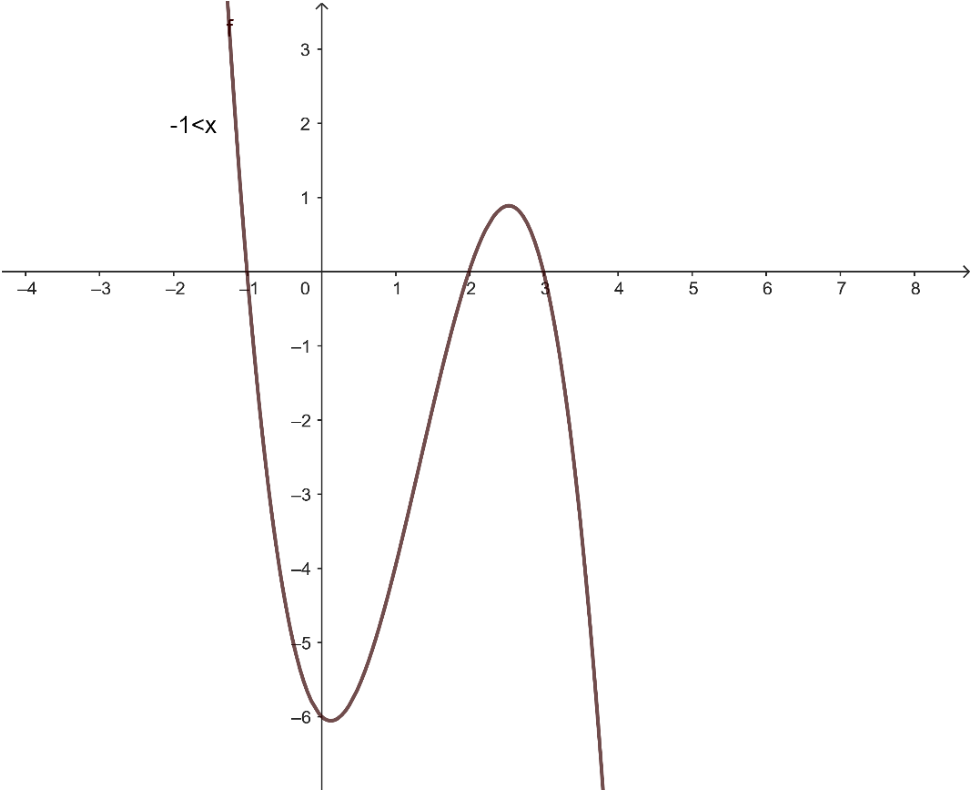
\includegraphics[width=0.75\linewidth]{figures/fig3-5.png}
\end{center}
\figcaption{3.5}{\textit{Curve of} $-x^3 + 4x^2 - x - 6$}
\end{example}

What polynomial function is represented in the graph below?
\begin{enumerate}
  \item[a.] How many factors does it have?
  \item[b.] Share your answers with the class.
\end{enumerate}
\begin{center}
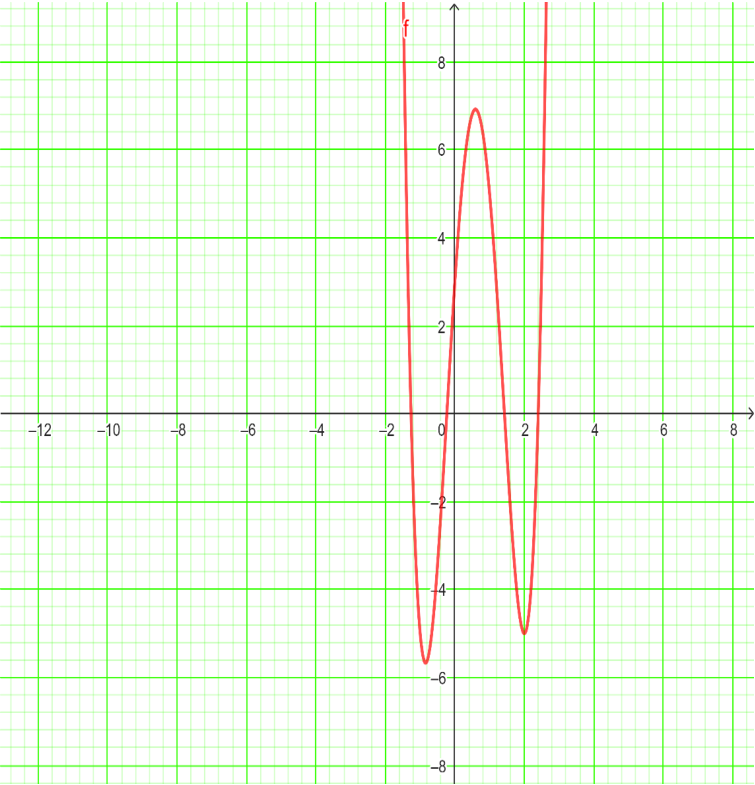
\includegraphics[width=0.6\linewidth]{figures/fig3-6.png}
\end{center}
\figcaption{3.6}{Graph of a polynomial function}

Remember that it is an important skill to be able to sketch graphs by hand.
However, when appropriate technology is there to assist. For example, you can
use apps or web-based programs such as GeoGebra, Demos, PhET Simulations
and Geometer's Sketch Pad.
